
\subsection{Induttanza per unità di lunghezza di una linea bifilare}
Una linea di trasmissione presenta solitamente quattro parametri: induttanza, capacità, 
resistenza e conduttanza verso il suolo per unità di lunghezza.
Si utilizzano solitamente le equazioni di propagazione provenienti dalle equazioni di Maxwell
complete.

\begin{figure}[H]
\centering
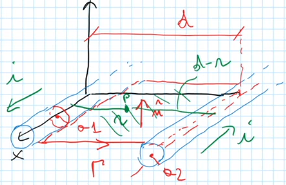
\includegraphics[width = 0.4\linewidth]{linea_bifilare_induttanza}
\end{figure}

Una linea bifilare può essere schematizzata mediante due conduttori cilindrici orientati 
nella stessa direzione, si possono supporre i raggi diversi  per completezza d'analisi
anche se solitamente avviene il contrario; la distanza fra gli assi è $d$.

La linea $\Gamma$ per il calcolo del flusso giace nel piano dei conduttori e la superficie
orlata è concorde all'asse $z$. La corrente percorrerà i conduttori in versi opposti.

Si determina il campo $\vec{B}$ con il PSE, le linee di campo prodotte da entrambi i 
conduttori saranno concordi alla superficie di controllo.
Sia $r$ la distanza del punto da un conduttore, la distanza rispetto all'altro conduttore
sarà $d-r$.
$$
\vec{B} = \frac{\mu_0}{2\pi } \frac{i}{r} \hat{n} + \frac{\mu_0}{2 \pi} \frac{i}{d-r} \hat{n}
$$

Il flusso sarà
$$
\Phi_\Gamma = \iint_{S_\gamma} \vec{B}\cdot\hat{n}dS = \int_0^l dx \int_{a_1}^{d-a_2} dr 
\frac{\mu_0}{2\pi} i \left( \frac{1}{r} + \frac{1}{d-r} \right) = l \frac{\mu_0}{2\pi}i \left( \left[\ln\left(r\right)\right]_{a_1}^{d-a_2}  + \ln\left[d-r\right]_{a_1}^{d-a_2} \right)
$$
$$
\Phi_\Gamma = l\frac{\mu_0}{2\pi} i \ln\left(\frac{(d-a_2)(d-a_1)}{a_1a_2}\right)
$$
Nell'ipotesi realistica in cui la distanza dei conduttori è molto maggiore del raggio degli 
stessi ($d\gg a_1a_2$)
$$
\frac{L}{l} = \frac{\Phi_\Gamma}{L\cdot i} \simeq \frac{\mu_0}{2\pi} \ln\left(\frac{d^2}{a_1a_2}\right)
$$

La capacità per unità di lunghezza di una linea bifilare è
$$
\frac{C}{l} = \frac{2\pi \varepsilon_0}{\ln\left(\frac{d^2}{a_1a_2}\right)}
$$

Analizzando la velocità di propagazione
$$
\frac{C}{l}\cdot\frac{L}{l} = \mu_0\varepsilon_0 = \frac{1}{c^2}
$$

\subsection{Induttanza di un solenoide toroidale a sezione rettangolare}
Sia $z$ l'asse di rotazione di una sezione rettangolare che genera un solido di rivoluzione
avvolto ergodicamente con un conduttore che realizza $N$ spire percorse dalla corrente $i$.

\begin{figure}[H]
\centering
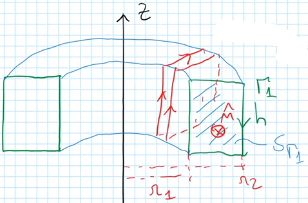
\includegraphics[width = 0.4\linewidth]{induttanza_toroide}
\end{figure}

Si suppone di applicare ad una singola spira la superficie piana di controllo attraverso la
quale si calcolerà il flusso, orientata concordemente al verso della corrente.
$$
\left.\vec{B}\right|_{S_{\Gamma_1}} = \frac{\mu_0}{2\pi r} Ni \hat{n}
$$
Il flusso attraverso una spira $\Gamma_1$ sarà
$$
\Phi_{\Gamma_1} = \int_0^h dz \int_{r_1}^{r_2} \frac{\mu_0}{2\pi r} N i dr = h \frac{\mu_0}{2\pi} Ni \ln\left(\frac{r_2}{r_1}\right)
$$
Quello totale sarà il prodotto del flusso di una spira per il numero di spire
$$
\Phi_{\text{tot}} = N\Phi_{\Gamma_1} = h \frac{\mu_0}{2\pi} N^2 i \ln\left(\frac{r_2}{r_1}\right)
$$
L'induttanza
$$
L = \frac{\Phi_{\text{tot}}}{i} = h \frac{\mu_0}{2\pi} N^2 \ln\left(\frac{r_2}{r_1}\right)
$$

\newpage
\subsection{Mutua induzione di due avvolgimenti toroidali concentrici}
Ad esempio nella realizzazione dei trasformatori gli avvolgimenti vengono posti l'uno 
sull'altro. In figura è rappresentata una singola spira degli avvolgimenti concentrici.
\begin{figure}[H]
\centering
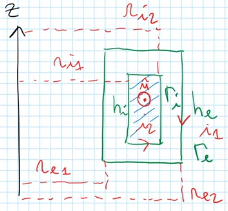
\includegraphics[width = 0.4\linewidth]{induttanza_avvolgimenti_concentrici}
\end{figure}
Le equazioni del problema sono le seguenti
\begin{align*}
\Phi_1 &= L_{11}i_1 + L_{12}i_2 \\
\Phi_2 &= L_{21}i_1 + L_{22}i_2
\end{align*}

Si calcola il flusso concatenato con l'avvolgimento interno e generato da quello 
esterno, $\Phi_{21} = \Phi_{\Gamma_i}$
$$
\Phi_{\Gamma_i} = \iint_{S_{\Gamma_i}} \vec{B}\cdot\hat{n}dS
$$
ma 
$$
\vec{B} = \frac{\mu_0}{2 \pi r} N_1 i_1 (-\hat{n}) \qquad r\in (r_{e_1},r_{e_2})
$$
$$
\Phi_{\Gamma_i} = h_i \int_{r_{i_1}}^{r_{i_2}}dr \left(-\frac{\mu_0}{2\pi r} N_1 i_1\right) =
-h_i \frac{\mu_0}{2 \pi} \ln\left(\frac{r_{i_2}}{r_{i_1}}\right) N_1 i_1
$$
Il flusso totale concatenato all'avvolgimento interno (2) è dunque
$$
\Phi_{\text{tot}_i} = N_2 \Phi_{\Gamma_i} = -h_i \frac{\mu_0}{2 \pi} N_1N_2 \ln\left(\frac{r_{i_2}}{r_{i_1}}\right) i_1 = L_{21} i_1
$$

\newpage
\section{Campo magnetico in presenza di mezzi materiali}
Si tenterà di modellare il campo magnetico nella materia utilizzando il fenomeno
delle correnti molecolari, dette correnti ``amperiane'' dovute al moto
degli elettroni nei loro orbitali, previsti dal modello della meccanica quantistica.
Ha ancora senso da un punto di vista classico valutare la media in piccola scala di questo 
fenomeno. 
Si immagina la materia come una distribuzione continua di dipoli elementari.

Si considera un atomo di idrogeno, composto da un protone e un elettrone, si suppone
un orbita circolare dell'elettrone (ATTENZIONE NON È UN MODELLO ACCURATO DEL MOTO DEGLI ELETTRONI MA FORNISCE BUONI RISULTATI DAL PUNTO DI VISTA DEL CAMPO MAGNETICO).
\begin{figure}[H]
\centering
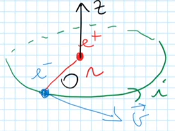
\includegraphics[width = 0.3\linewidth]{orbita_elettrone}
\end{figure}
Si associa all'elettrone una corrente elettrica di intensità
$$
i = \frac{e^-}{T}
$$
dove $e^-$ è la carica dell'elettrone e $T$ il periodo di rivoluzione dell'orbita di raggio $r$.
Il momento magnetico di una spira circolare elementare è 
$$
\vec{\mu} = i \pi r^2 \vec{e}_z \Rightarrow \left|\vec{\mu}\right| = \frac{e^-}{\frac{2\cancel{\pi}}{\omega}}\cancel{\pi} r^2 = \frac{e^-}{2}\omega r^2
$$

Il momento angolare dell'elettrone è 
$$
\vec{L}_e = \vec{r} \times m_e \vec{v}
$$
il cui modulo
$$
\left|\vec{L}_e\right| = r m_e v = m_e \omega r^2
$$
confrontando i due termini 
$$
\left|\vec{\mu}\right| = \mu_B = \frac{e^-}{m_e\cdot 2} L_e = \frac{\gamma}{2}L_e
$$
con il termine $\gamma$ chiamato fattore \textit{giromagnetico} dell'elettrone pari al 
rapporto fra la carica e la massa dell'elettrone, una costante fondamentale 
dell'elettromagnetismo.
\begin{align*}
e^- &= \SI{-1.6e-19}{\coulomb}\\
m_e & = \SI{9.11e-31}{\kilo\gram} \\
\gamma &= \SI{-1.76e11}{\coulomb\per\kilo\gram}
\end{align*}
1:06:44
